\section{Mereology}
\label{section:Mereology}
Mereology is the logical study on the semantics of parthood.
\textit{"As a formal theory, mereology is simply
an attempt to set out the general principles underlying the relationships between a whole and its constituent parts [...]"} \cite{DBLP:journals/dke/Varzi96}.
Achille C. Varzi describes a collection of formal theories, i.e. sets of distinct axioms, of mereology in \cite{DBLP:journals/dke/Varzi96}, which will be summarized in this section.

The first part of this section will just introduce the axioms of mereology.
Then, at the end of this section, we will use these axiom to build some of the theories described in \cite{DBLP:journals/dke/Varzi96}.
Note, that the terms relation, relationship and predicate may be used synonymously throughout this section.


\subsection{Parthood}
\label{subsection:Parthood}
First we define the intuitive notion of the parthood relationship:
\begin{definition}[$\partOf$]
Let $x$ and $y$ objects of interest.
We define:
\begin{align}
x \partOf y
:\Leftrightarrow
x \text{ is a constituent part of } y
\end{align}
\end{definition}
We further assume, that $\partOf$ satisfies the following properties:
\begin{align}
&\text{(P1)}
\qquad x \partOf x 
&\qquad \text{(Reflexivity)}
\\
&\text{(P2)}
\qquad x \partOf y \wedge y \partOf x \rightarrow x = y
&\qquad \text{(Antisymmetry)}
\\
&\text{(P3)}
\qquad x \partOf y \wedge y \partOf z \rightarrow x \partOf z
&\qquad \text{(Transitivity)}
\end{align}
Thus, $\partOf$ induces a partial order of things.

However, since the reflexive parthood may be to week for some cases, we also define a stricter, irreflexive parthood relationship as follows:
\begin{align}
x \properPartOf y
:\Leftrightarrow
x \partOf y \wedge \neg(y \partOf x)
\end{align}
Proper parthood induces a strict partial order of things.

In addition to the relationships above we introduce the following predicates in order to provide a more concise notation:
\begin{align}
x \overlaps y
&:\Leftrightarrow
\exists z : z \partOf x \wedge z \partOf y
&\qquad \text{(Overlap)}
\\
x \underlaps y
&:\Leftrightarrow
\exists z : x \partOf z \wedge y \partOf z
&\qquad \text{(Underlap)}
\end{align}
Overlap models situations, where two things share at least on distinct part.
Underlap models situations, where two things belong to the same distinct whole.

\subsection{Supplementation}
\label{subsection:Supplementation}
The fourth axiom, which can be assumed in an universe described by means of mereology, is the supplementation axiom.
It models the effects of situations more precisely, where one thing is not part of another.
Namely, if this is the case, a third thing may exist, which is part of the former but not part of the latter.
\begin{align}
&\text{(P4)}
\qquad
\neg(x \partOf y) \rightarrow \exists z (z \partOf x \wedge \neg(z \overlaps y))
\end{align}
The supplementation axiom reads: If a thing $x$ is not part of another thing $y$, then at least one part of $x$ does not share further parts with $y$.
Figure \ref{fig:SupplementaitonAxiomExample} exemplifies the supplementation axiom.

\begin{figure}[h!]
\begin{center}
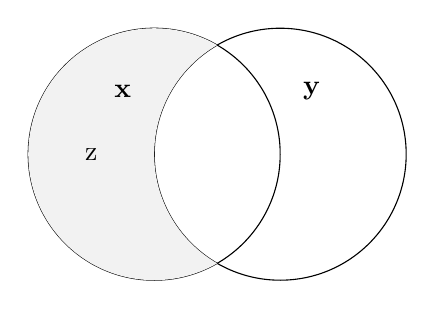
\begin{tikzpicture}[scale=0.8]
\draw(1,1)circle(2 and 2);
\draw(3,1)circle(2 and 2);
\scope
\clip (-1,-1) rectangle (3,3)
	  (3,1) circle (2 and 2);
\fill[gray!10] (1,1) circle (2 and 2);
\endscope
\draw(0.5,2)node{\textbf{x}};
\draw(3.5,2)node{\textbf{y}};
\draw(0,1)node{z};
\end{tikzpicture}
\end{center}
{
\scriptsize 
This Venn-style diagram exemplifies the supplementation axiom:
$x$ is not part of $y$.
Thus, $x$ contains a part $z$ (emphasized as gray area), which shares no further parts with $y$
}
\caption{Example for the Supplementation Axiom}
\label{fig:SupplementaitonAxiomExample}
\end{figure}

%\usetikzlibrary{calc}
%\begin{tikzpicture}[scale=0.8]
%\draw(4,3)circle(5 and 3)node(A){Text A};
%\draw(8,6)circle(5 and 3)node(B){Text B};
%\draw(10,2.5)circle(5 and 3)node(C){Text C};
%\begin{scope}
%\clip(4,3)circle(5 and 3);
%\clip(8,6)circle(5 and 3);
%\clip(10,2.5)circle(5 and 3);
%\filldraw[yellow!80](0,0)rectangle(10,10);
%\end{scope}
%\node at ($0.33*(A)+0.33*(B)+0.33*(C)$){Text M};
%\end{tikzpicture}

\ToDo{add paragraph explaining "strong" and "weak" supplementation}

One can also observe from figure \ref{fig:SupplementaitonAxiomExample}, that the supplementation axiom can be interpreted as analogue to set-theoretic difference.

\subsection{Sum}
\label{subsection:Sum}
\begin{align}
&\text{(P5)}
\qquad
\begin{split}
&x \underlaps y 
\\&\rightarrow
\exists z \forall w (x \overlaps z \leftrightarrow (w \overlaps x \vee w \overlaps y))
\end{split}
\end{align}

\subsection{Universal Top \& Bottom}
\label{subsection:UniversalTopAndBottom}

\subsection{Mereology Theories}
\label{subsection:MereologyTheories}